\documentclass{article}
\usepackage[UTF8]{ctex}
\usepackage{algorithm}
\usepackage{algpseudocode}
\usepackage{amsmath}
\usepackage{fancyhdr}
\usepackage{geometry}
\usepackage{tikz}
\usepackage{sectsty}

\geometry{left=2cm, right=2cm, top=2cm, bottom=2cm}
\sectionfont{\fontsize{12pt}{15pt}\selectfont}

\title{机器学习——第二次作业}
\author{Koorye}
\date{2024年3月8日}

\pagestyle{fancy}
\fancyhead[L]{机器学习——第二次作业}
\fancyhead[R]{Koorye}
\fancyfoot[R]{基于\LaTeX 排版制作}

\begin{document}
\maketitle
\thispagestyle{fancy}

\section{请给出梯度下降算法的流程,如果采用固定学习率,学习率过大或过小会造成什么后果?}

梯度下降法是一种用于可微函数的最优化方法。通过计算损失函数的梯度,并向梯度负方向移动来逼近损失函数的最小值,从而学习最优的目标函数。梯度下降法的详细流程可以表示为算法\ref{alg:gd}。

\begin{algorithm}
    \caption{梯度下降法}
    \label{alg:gd}
    \begin{algorithmic}[1]
        \Require 输入数据集$X$,标签集$Y$,目标函数$f(\cdot,\theta),$损失函数$L(\cdot,\cdot)$,学习率$\eta$,精度$\epsilon$。
        \Ensure 最优参数$\theta$。
        \State 随机初始化$\theta$。
        \While{损失函数$L(\hat{Y},Y)>\epsilon$}
            \State $\hat{Y}\gets f(X,\theta)$, // 计算预测值
            \State $\nabla_\theta\gets\frac{\partial L(\hat{Y},Y)}{\partial\theta}$, // 计算梯度
            \State $\theta\gets\theta-\eta\nabla_{\theta}$。 // 更新参数
        \EndWhile
    \end{algorithmic}
\end{algorithm}

上述算法描述了一个最简单的梯度下降流程,没有考虑学习率等动态变化或早停等策略。当学习率过大时,可能会导致预测值来回跳动,使得梯度下降法无法收敛,甚至发散。当学习率过小时,可能会导致梯度下降法收敛速度过慢,甚至陷入局部最优解而无法收敛到更好的结果。

\section{在机器学习中根据使用训练数据的不同运用梯度下降的方式有哪些?各有什么优缺点?列举出几种梯度下降的改进方法(名称即可)。}

不同的梯度下降方式有:
\begin{enumerate}
    \item \textbf{批量梯度下降(Batch Gradient Descent)}:使用全部训练数据计算梯度。其优点是收敛稳定,效率更高,因为它计算所有样本的全局梯度。缺点是计算量大,学习速度较慢。
    \item \textbf{随机梯度下降(Stochastic Gradient Descent)}:使用单个样本计算梯度。其优点是更新速度快,计算量小。缺点是准确度下降,因为它只计算单个样本的局部梯度;其次收敛不稳定,效率低。
    \item \textbf{小批量梯度下降(Mini-batch Gradient Descent)}:使用一小部分样本计算梯度。结合批量梯度下降和随机梯度下降的优点,优化速度快,计算量小且比较稳定。缺点是仍然可能振荡不稳定,且batch size对性能有较大影响。
\end{enumerate}

\section{什么是最小二乘回归(Least Squares Regression),写出它的损失函数,试用从概率观点给出解释。请采用最小二乘回归用直线拟合下面三个数据点 :(1, 0.9)、 (0, 0.1)、 (2, 2)。}

最小二乘回归是一种线性回归方法,通过最小化残差平方和来拟合数据。其损失函数可以表示为:

\begin{equation}
    L(\hat{Y},Y)=\sum_{i=1}^{n}(\hat{y}_i-y_i)^2=\sum_{i=1}^{n}(y_i-\theta^T\phi(x_i))^2,
\end{equation}

其中$\phi(\cdot)$是任意基函数。

下面是最小二乘回归概率观点的解释。从极大似然的角度解释最小二乘回归,可以认为数据点$Y_i$是由某种模型$f(X,\theta)$加上高斯噪声$\epsilon_i$得到的,即:

\begin{equation}
    y_i=f(x_i,\theta)+\epsilon_i, \epsilon_i\sim N(0,\sigma^2).
\end{equation}

因此对于输入数据$X$和参数$\theta$,输出$Y$的概率分布即为:

\begin{equation}
    P(Y|X,\theta)=\prod_{i=1}^{n}\frac{1}{\sqrt{2\pi\sigma^2}}\exp\left(-\frac{(y_i-f(x_i,\theta))^2}{2\sigma^2}\right).    
\end{equation}

最大化该概率分布,即最大化概率分布函数的$\ln$值:

\begin{equation}
    \max\ln P(Y|X,\theta)=-\frac{n}{2}\ln(2\pi\sigma^2)-\frac{1}{2\sigma^2}\sum_{i=1}^{n}(y_i-f(x_i,\theta))^2.
\end{equation}

要求上式的最大值,即求下式最小值:

\begin{equation}
    \min\sum_{i=1}^{n}(y_i-f(x_i,\theta))^2.
\end{equation}

该式即为最小二乘回归的损失函数。

下面是数据点的拟合过程。设模型为$\hat{y_i}=wx_i+b$,要学习的参数为$w$,$b$。则最小二乘回归的损失函数为:

\begin{equation}
    L(w,b)=\sum_{i=1}^{n}(y_i-wx_i-b)^2.
\end{equation}

令上式对$w$,$b$的偏导数为0,即:

\begin{equation}
    \begin{cases}
        \frac{\partial L(w,b)}{\partial w}=-2\sum_{i=1}^{n}x_i(y_i-wx_i-b)=0. \\
        \frac{\partial L(w,b)}{\partial b}=-2\sum_{i=1}^{n}(y_i-wx_i-b)=0.
    \end{cases}
\end{equation}

联立两式,解得:

\begin{equation}
    \begin{cases}
        w=\frac{\sum_i(x_i-\overline{x})(y_i-\overline{y})}{\sum_i{(x_i-\overline{x})^2}}. \\
        b=\overline{y}-w\overline{x}.
    \end{cases}
\end{equation}

代入数据$(1,0.9),(0,0.1),(2,2)$得:

\begin{equation}
    \begin{cases}
        w=\frac{(1-1)(0.9-1)+(0-1)(0.1-1)+(2-1)(2-1)}{(1-1)^2+(0-1)^2+(2-1)^2}=\frac{0.9+1}{2}=0.95. \\
        b=1-0.5*1=0.05.
    \end{cases}
\end{equation}

即$\hat{y_i}=0.95x_i+0.05$,如图\ref{fig:lsr}所示。

\begin{figure}[h]
\centering
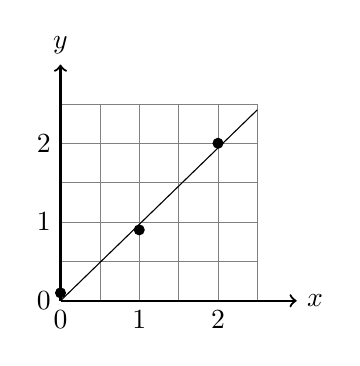
\begin{tikzpicture}
    \draw[help lines,step=0.5](0,0) grid (2.5,2.5);
    \draw[thick,->](0,0)--(3,0) node[right]{$x$};
    \draw[thick,->](0,0)--(0,3) node[above]{$y$};
    \foreach \x in {0,1,2}
        \draw (\x,0) node[below]{$\x$};
    \foreach \y in {0,1,2}
        \draw (0,\y) node[left]{$\y$};
    \fill (1,0.9) circle (2pt);
    \fill (0,0.1) circle (2pt);
    \fill (2,2) circle (2pt);
    \draw (0,0) -- (2.5,2.425);
\end{tikzpicture}
\caption{最小二乘回归拟合结果}
\label{fig:lsr}
\end{figure}

\section{什么是岭回归(Ridge Regression),写出它的损失函数,试用从贝叶斯观点给出解释,并说明它的优点。}

岭回归是一种线性回归方法,通过最小化残差平方和加上L2正则项来拟合数据。其损失函数可以表示为:

\begin{equation}
    L(\hat{Y},Y)=\sum_{i=1}^{n}(\hat{y}_i-y_i)^2+\lambda\sum_{j=1}^{m}\theta_j^2\propto\frac12\sum_{i=1}^n(\hat{y}_i-\theta^T\phi(x_i))^2+\frac\lambda 2\theta^T\theta.
\end{equation}

从贝叶斯观点解释岭回归,认为$P(Y|X,\theta)$的先验分布服从高斯分布:

\begin{equation}
    P(\theta)=\mathcal{N}(0,\Sigma_0)\propto\frac{1}{\sqrt{(2\pi)^m|\Sigma_0|}}\exp(-\frac12\theta^T\Sigma_0^{-1}\theta).
\end{equation}

另外,$P(Y|X,\theta)$服从高斯分布:

\begin{equation}
    P(Y|X,\theta)=\mathcal{N}(\theta^Tx,\Sigma_1)\propto\frac{1}{\sqrt{(2\pi)^n|\Sigma_1|}}\exp(-\frac12(Y-\theta^Tx)^T\Sigma_1^{-1}(Y-\theta^Tx)).
\end{equation}

$\theta$的后验分布即为:

\begin{equation}
    P(\theta|Y,X)\propto P(Y|X,\theta)P(\theta).
\end{equation}

最大化后验概率即:

\begin{equation}
\begin{split}
    \max_\theta P(\theta|Y,X)\propto\max_\theta\ln P(Y|X,\theta)P(\theta)=\max_\theta\ln[P(Y|X,\theta)+\ln P(\theta)] \\
    =\max_\theta\ln\frac{1}{\sqrt{(2\pi)^m|\Sigma_0}}-\frac12\theta^T\Sigma_0^{-1}\theta+\ln\frac{1}{\sqrt{(2\pi)^n|\Sigma_1|}}-\frac12(Y-\theta^Tx)^T\Sigma_1^{-1}(Y-\theta^Tx).
\end{split}
\end{equation}

相当于最小化下式:

\begin{equation}
    \min_\theta\frac12\theta^T\Sigma_0^{-1}\theta+\frac12(Y-\theta^Tx)^T\Sigma_1^{-1}(Y-\theta^Tx)=\min_\theta(Y-\theta^TX)^2+\lambda\theta^T\theta.
\end{equation}

该式即为岭回归的损失函数。

岭回归的优点有:
\begin{enumerate}
    \item 限制模型的复杂度,防止过拟合,提高模型的泛化能力。
    \item 还可以求解奇异矩阵的逆矩阵,容易获得闭式解。
    \item 将确定基函数参数的问题转换为确定岭回归超参数$\lambda$的问题,可以通过交叉验证等方法选择最优的超参数,更容易确定最优解。
\end{enumerate}

\end{document}